\section{Related Work}
\label{section:related-work}

\subsection{The Hague}
\textcite{van-oort-2015} analyzed the bus and tram network of The Hague, Netherlands for their research of developing a tool that provides customers with predictions regarding the punctuality of their trips. First, they explained various reasons for delays, dividing them into \textit{internal} and \textit{external} reasons. Internal meaning that the problem originates from the network operation itself, for example, schedule quality, infrastructure design or driver behavior. External reasons on the other hand include things that the network operator has no influence over, such as traveler behavior, other traffic or simply bad weather conditions \autocite[372--374]{van-oort-2015}.

After collecting data over several months using a newly available open data \ac{API} provided by the Dutch government, the authors analyzed and visualized that data in varying degrees of detail. For the first visualization, as seen in \cref{fig:van-oort-1}, they plotted all recorded trips of a single transit line on a line diagram, with stops on the x-axis and delay in minutes on the y-axis. This diagram shows good general punctuality and indicates that there are multiple stations where vehicles arrive early and wait for their scheduled departure. In a second line diagram, the authors instead showed the interval in minutes on the y-axis. Besides absolute delay, this is an important measure as a transit line with steady delays, yet high-frequency intervals are still desirable for passengers. Both diagrams together show that in the last third of the route, delays accumulate the most, leading to both higher absolute delays and increased intervals. \autocite[378]{van-oort-2015}.

\begin{figure}[h]
	\centering
	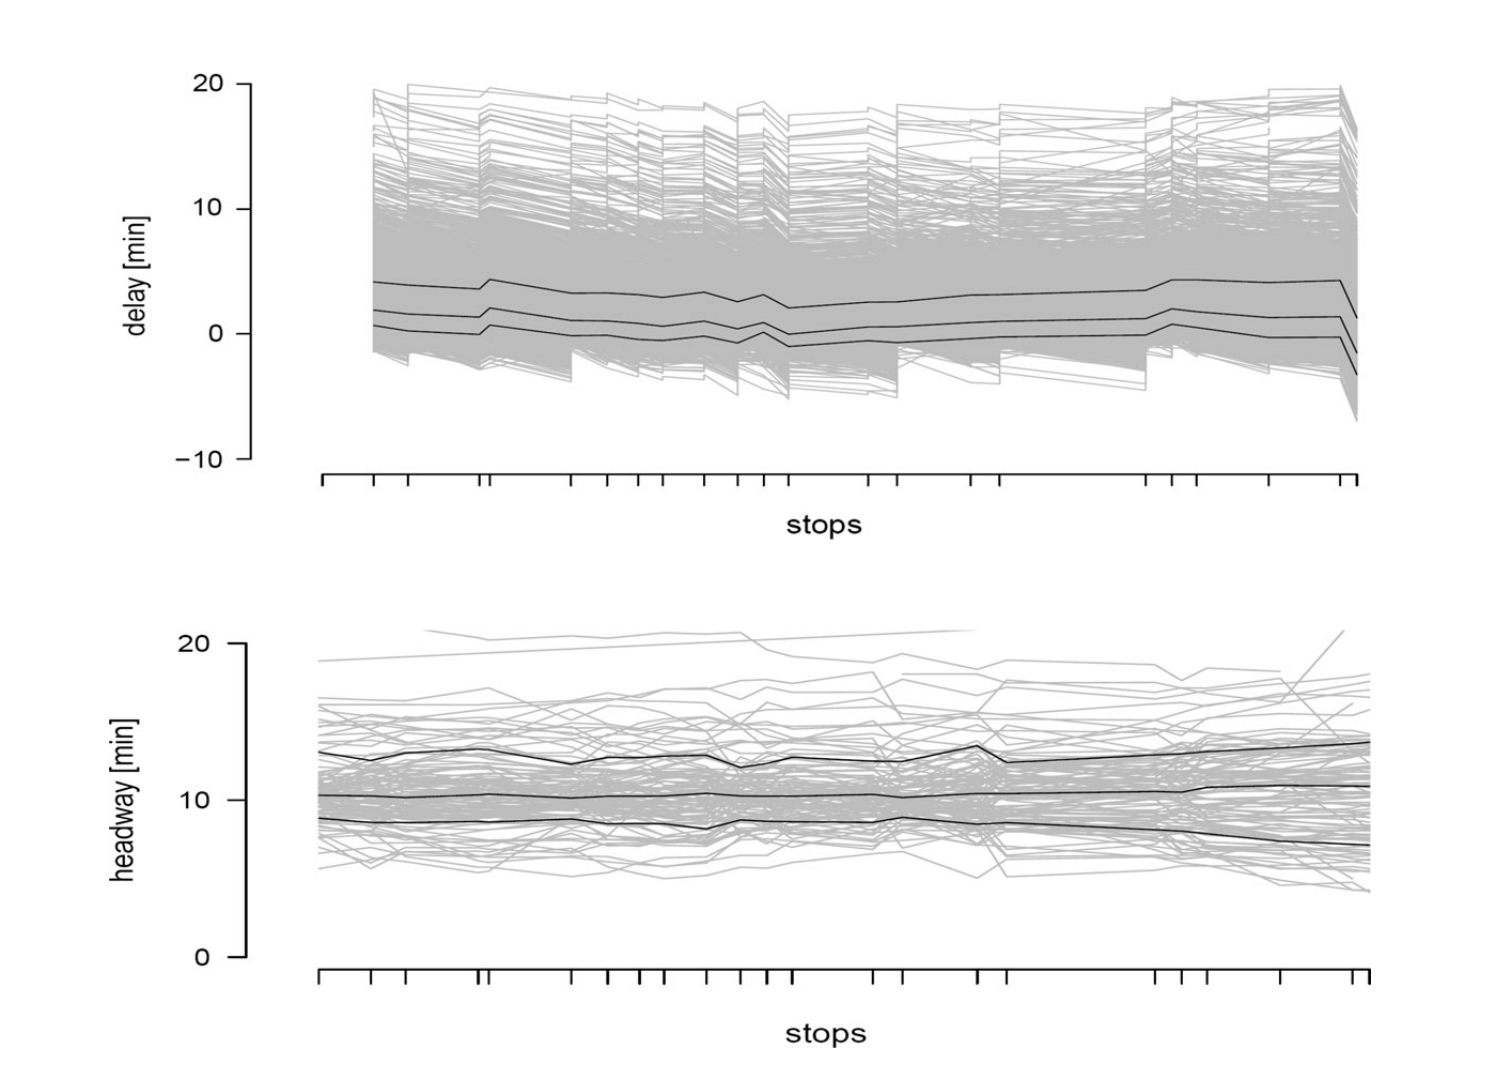
\includegraphics[width=0.8\textwidth]{van-oort-1}
	\caption{Vehicle delays (upper) and headways (lower) along a single route \autocite[378]{van-oort-2015}}
	\label{fig:van-oort-1}
\end{figure}

In \cref{fig:van-oort-2}, one can see a network-wide visualization, where each station is colored in a gradient from green to red, representing the average delay recorded at that station. It shows that overall there are only a few problem areas which are mostly series of stops where delays may accumulate. Interestingly, there are stations with a negative average delay, meaning an earlier-than-planned arrival. This effect can in certain cases be an expected result of including a leeway in schedules for important transfer hubs. If not intentional, such early arrivals can simply be solved by updating scheduled departure data \autocite[379--380]{van-oort-2015}.

\begin{figure}[h]
	\centering
	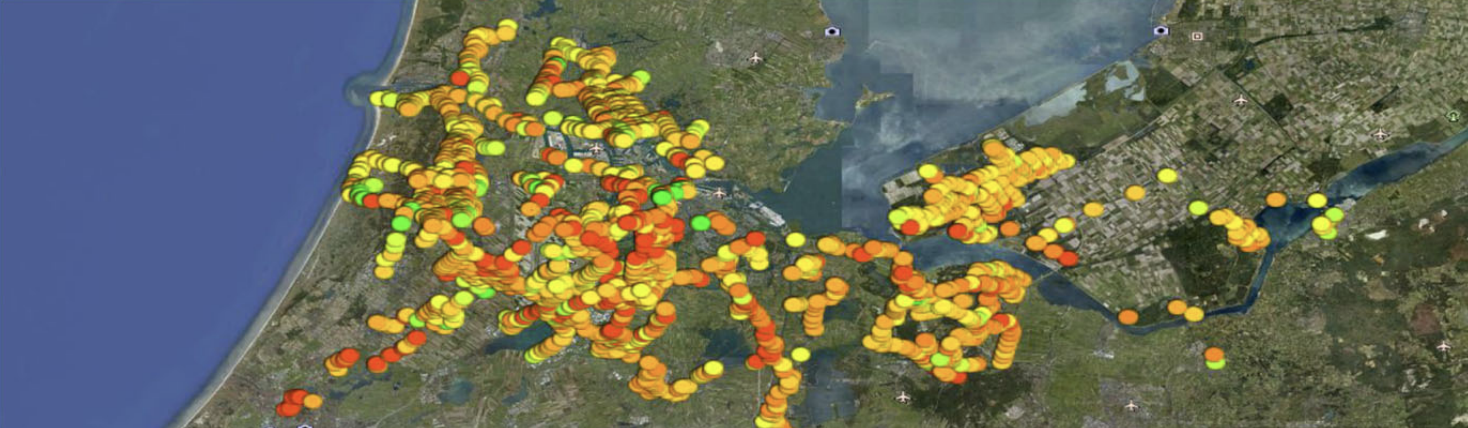
\includegraphics[width=0.9\textwidth]{van-oort-2}
	\caption{Average delay per stop (green early, yellow on time, red late) \autocite[379]{van-oort-2015}}
	\label{fig:van-oort-2}
\end{figure}

After this static analysis of historical data, the authors fitted the data to a normal distribution in order to provide passengers with so-called \textit{enriched travel advice}, where predictions based on said distribution are added to trip planning results. This information includes probabilities of delays, early departures or transfer feasibility. Additionally, they developed a tool for a more scientific analysis of collected data. This software was used on another data set from the transit network of Utrecht and was able to detect multiple bottlenecks in the network, for example, long dwell time on bus routes \autocite[380--387]{van-oort-2015}.

\subsection{Portland}

In 1993, \textcite{strathman-1993} presented a baseline study of the Portland metropolitan area transit network as part of an operations control plan implemented by the city's transit agency \textit{Tri-Met}. This plan aimed to improve the growing challenges the network was facing regarding service reliability. Like \textcite{van-oort-2015}, the authors state that for short intervals, passengers do not care about vehicles running exactly on time, but rather whether the service runs regularly and reliably. In addition to grouping causes for delays into internal and external ones, the authors divide possible countermeasures into short-term and long-term actions. Short-term actions are ones to counter unanticipated delays such as holding vehicles at a stop in case of early arrival or adding additional vehicles to a route. Long-term actions on the other hand are helpful for systemic delays which are not caused by a single unexpected event. Examples include improving driver behavior through additional training or a reward system for good on-time performance. Additionally, the schedule itself can be the root cause and a redesign with longer run times or longer layover times at the end of lines may be the solution for consistent delays. The authors also state that a more complex network with longer routes generally results in worse on-time performance than one with short routes and only a few stops. Also, lines where the highest loads occur at the first few stations are more likely to show higher delay rates. As a result, public transport providers have to balance satisfying the demands of passengers and thus network complexity with on-time performance, taking various factors such as efficient use of resources into consideration. \autocite[93--94]{strathman-1993}.

The study was conducted by manually recording arrival times on 200 trips on 59 different bus lines in the Portland metropolitan area, resulting in a total of 1552 recorded bus arrival times. Of those, 1360 or 87.6\% were punctual, with an arrival considered punctual if it falls within a range of being one minute early to five minutes late. The authors found that driver experience has a measurable effect on on-time performance, with part-time drivers being more prone to late arrivals than their full-time colleagues. Furthermore, they confirmed that early arrivals and delays occur more often during afternoon peak hours. Interestingly, they did not observe this effect for morning peak hours. In fact, arrivals were more likely to be early than late if they did not follow the schedule, indicating that planners overcompensated for morning rush hour traffic by increasing running more than necessary \autocite[97--99]{strathman-1993}.

\subsection{New York City}

A team of researchers from the Data, Research, Development (DRD) department of the New York City Transit Authority developed a tool for visualizing problem areas in New York's subway system. It detects areas where trains run slower than normal or show longer than normal intervals between trains. In addition to highlighting the results with a severity level, an interactive map display the locations of trains in real-time. This interactive map is used by the communications team in order to inform customers via social media channels about those problems occurring in the network. While there were similar tools already available for the New York transit network, these tools had significant limitations such as only allowing to view one direction of one line at a time. This required the monitoring staff to switch between the lines constantly to keep an overview. \autocite[1--3]{caspari-2021}

To gather the required train location data, the authors used a combination of real-time station arrival feeds and data provided by the signaling system. To compare running times between two stations or signaling segments, they relied on manual recordings by the transit authority rather than schedule data. They found that actual running times can deviate from scheduled ones and thus using schedules alone would result in less accurate calculations \autocite[4]{caspari-2021}. Both large intervals and slow trains are calculated and displayed on multiple levels of detail. Longer-than-normal intervals are first calculated for stops or track segments, then aggregated into bigger areas of three or more stops if applicable. For slow trains it is done similarly, ranging from single stuck trains to entire areas consisting of multiple stations where trains run significantly slower than expected. All results are then categorized into \textit{moderate}, \textit{severe} and \textit{very severe} problems, aiming to provide passengers with consistent information and suggested actions depending on the severity level \autocite[6--7]{caspari-2021}.

The interactive map that \textcite{caspari-2021} developed needed to cater to various needs, providing both an overview to detect emerging problem areas and the ability to see detailed information about a specific problem. The solution was a zoomable map, in addition to a text-based sidebar and tooltips for stations and line segments. Additional features include different available themes for severity levels, dark and light themes for the entire app and a text-only mode that displays the data in a tabular layout instead of the interactive map \autocite[8--9]{caspari-2021}. The tool was developed for more than one year and is in successful use since then. Being entirely web-based, it even allowed for easy access during the COVID-19 pandemic for the communications personnel \autocite[11]{caspari-2021}.

\subsection{Stochastic models}

Various authors have studied the fitting of delay data to statistical distribution models in order to be able to make predictions over possible future delays. \textcite{yuan-2008} found that while other distributions may provide more flexibility and adjustable parameters, a negative exponential distribution is most of the time a valid and easy-to-understand distribution to model both arrival and departure delays \autocite[173--174]{yuan-2008}. Depending on the data set and the exact delay variable being measured, other distributions might fit better. For example, \textcite[90]{goverde-2013} fitted their data of trains arriving in Utrecht to a Weibull distribution, which is a distribution that receives multiple input parameters and---depending on one of those parameters---can result in an exponential distribution too \autocite[88]{hallinan-1993}. \textcite[61]{yuan-2006} confirmed that the Weibull distribution most of the time offers the best fit. In some cases, however, other distributions such as beta, gamma or log-normal distributions model departure delays the best \autocite[61]{yuan-2006}.

\subsection{Data availability}

\subsubsection{\acf{HAFAS}}

In Germany, Austria and Switzerland but also other European countries, \acs{HAFAS}, short for \textit{\acl{HAFAS}} (HaCon Timetable-Information-System), is a popular system for retrieving timetable information as well as intermodal journey planning. It is developed by a subsidiary of Siemens and available since the late 1980s, and with that one of the first tools on the market, promising an algorithm that performs route calculation in less than six seconds. Each public transport company gets its own \ac{HAFAS} deployment, which all share common terminology and endpoints, but can however use custom configurations and feature availability. While the endpoints are usually not openly documented by the respective companies, they do not restrict access using \ac{API} tokens or similar measures and are therefore easily accessible \autocites{computerwoche-1988}{redmann-2023b}.

For this thesis, the  \ac{HAFAS} endpoint by \ac{VOR}, the transport authority of the eastern regions of Austria, was used for collecting the necessary data. While the \ac{API} itself returns data in the  \ac{HAFAS} Raw Data Format, the JavaScript library \textit{hafas-client} converts this into the much easier-to-work-with \ac{FPTF}, which is inspired by the widely used \ac{GTFS} format and uses \ac{JSON} as its serialization format \autocite{redmann-2023a}.

The library provides a multitude of endpoints, both for station and trip data. Aside from fetching information about a stop or station, the \texttt{nearby} endpoint for example can retrieve all locations that are within a given walking distance in minutes, which is especially useful for building consumer-facing public transport applications. It also includes endpoints for journey planning between two given locations. Similar to \texttt{nearby}, the \texttt{reachableFrom} endpoint returns all stations that are reachable from another station, but instead of walking distance public transport journeys are calculated. Another endpoint that provides opportunities for interesting applications is \texttt{radar}, which returns the locations of all vehicles within a given radius. While location data is not available for all vehicles, this can certainly be used as a foundation for appealing visualizations. The two most important endpoints for this thesis however are \texttt{arrivals} and \texttt{departures}, which provide accurate real-time data for one or more given station(s). In addition to planned and actual arrival/departure times, they also calculate the difference, providing the consumer with a ready-to-use delay value in seconds \autocites{redmann-2023a}{redmann-2023c}.

\subsubsection{\acf{GTFS}}

\ac{GTFS} is a format specification initially developed by Google which later---after its widespread usage in many non-Google systems---has been renamed from \textit{Google Transit Feed Specification} to \textit{General Transit Feed Specification}. It allows public transport agencies to offer their data in a unified format, understood by various consumer applications, ranging from visualization tools to trip-planning mobile applications. The core of \ac{GTFS} is a static feed of text files that contain the whole schedule and additional information about the network. The \ac{GTFS} reference document specifies five required files: \texttt{agency.txt}, \texttt{stops.txt}, \texttt{routes.txt}, \texttt{trips.txt} and \texttt{stop\_times.txt}. One can see that the structure of the data is similar to \ac{HAFAS}. Routes are a group of trips that are offered to passengers as a line or service. Arrival and departure data for those trips are then collected in \texttt{stop\_times.txt} \autocite{gtfs-2022-schedule}.

In contrast to \ac{HAFAS} however, these static files do not provide any historical or real-time data, but instead the planned schedule at the time of publishing. For real-time data, there exists a special extension to \ac{GTFS} called \ac{GTFS} Realtime. As a data format, \ac{GTFS} Realtime uses Protocol Buffers, a language-agnostic serialization format developed by Google. As real-time updates naturally come with a significantly higher level of detail than static text files, the provided data structures are entirely different. Instead of static text files, messages such as \texttt{TripUpdate}, \texttt{VehiclePosition} or \texttt{StopTimeEvent} are exchanged between the feed provider and connected clients \autocite{gtfs-2022-realtime}. 

Since 2017, the city of Vienna provides \ac{GTFS} schedule data as part of the \textit{Open Government Data} initiative. With its real-time extension, \ac{GTFS} would have been able to provide all the necessary data for this thesis, especially planned and actual departure data. However, as the \textit{hafas-client} library uses the \ac{JSON}-based \ac{FPTF} format instead of more complicated Protocol Buffers, \ac{HAFAS} was chosen as a primary data source instead of \ac{GTFS}.
